\documentclass[dvisvgm,hypertex,aspectratio=169]{beamer}
\usefonttheme{serif}

\usepackage{animate}
\usepackage{ifthen}


%%%%%%%%%%%%%%%%%%%%%%%%%%%%%%%%%%%%%%%%%%%%%%%%%%%%%%%%%%%%%%%%%%%%%%%%%%%%%%%
% PageDown, PageUp key event handling; navigation symbols
%%%%%%%%%%%%%%%%%%%%%%%%%%%%%%%%%%%%%%%%%%%%%%%%%%%%%%%%%%%%%%%%%%%%%%%%%%%%%%%
\usepackage[totpages]{zref}
\usepackage{atbegshi}
\usepackage{fontawesome}
\setbeamertemplate{navigation symbols}{}
\AtBeginShipout{%
  \AtBeginShipoutAddToBox{%
    \special{dvisvgm:raw
      <defs>
      <script type="text/javascript">
      <![CDATA[
        document.addEventListener('keydown', function(e){
          if(e.key=='PageDown'){
            \ifnum\thepage<\ztotpages
              document.location.replace('\jobname-\the\numexpr\thepage+1\relax.svg');%
            \fi
          }else if(e.key=='PageUp'){
            \ifnum\thepage>1
            %document.location.replace('\jobname-\the\numexpr\thepage-1\relax.svg');%
              document.location.replace('\jobname-\makeatletter\@anim@pad{2}{\thepage-1}\makeatother\relax.svg');%
            \fi%
          }
        });
      ]]>
      </script>
      </defs>
    }%
  }%
  \AtBeginShipoutUpperLeftForeground{%
    \raisebox{-\dimexpr\height+0.5ex\relax}[0pt][0pt]{\makebox[\paperwidth][r]{%
      \normalsize\color{structure!40!}%
      \ifnum\thepage>1%
      \href{\jobname-\the\numexpr\thepage-1\relax.svg}{\faArrowLeft}%
      \else%  
        \textcolor{lightgray}{\faArrowLeft}%  
      \fi\hspace{0.5ex}%
      \ifnum\thepage<\ztotpages%
      \href{\jobname-\the\numexpr\thepage+1\relax.svg}{\faArrowRight}%
      \else%
        \textcolor{lightgray}{\faArrowRight}%  
      \fi%
      \hspace{0.5ex}%
    }}%
  }%  
}%
%%%%%%%%%%%%%%%%%%%%%%%%%%%%%%%%%%%%%%%%%%%%%%%%%%%%%%%%%%%%%%%%%%%%%%%%%%%%%%%

\usepackage{animate}
\usepackage{tikz}
\usepackage{circuitikz}

\author{Kjartan Halvorsen}
\date{2021-04-13}
\title{The induction motor - part 1}


\begin{document}

\maketitle


\begin{frame}{The induction motor}

  \begin{center}
    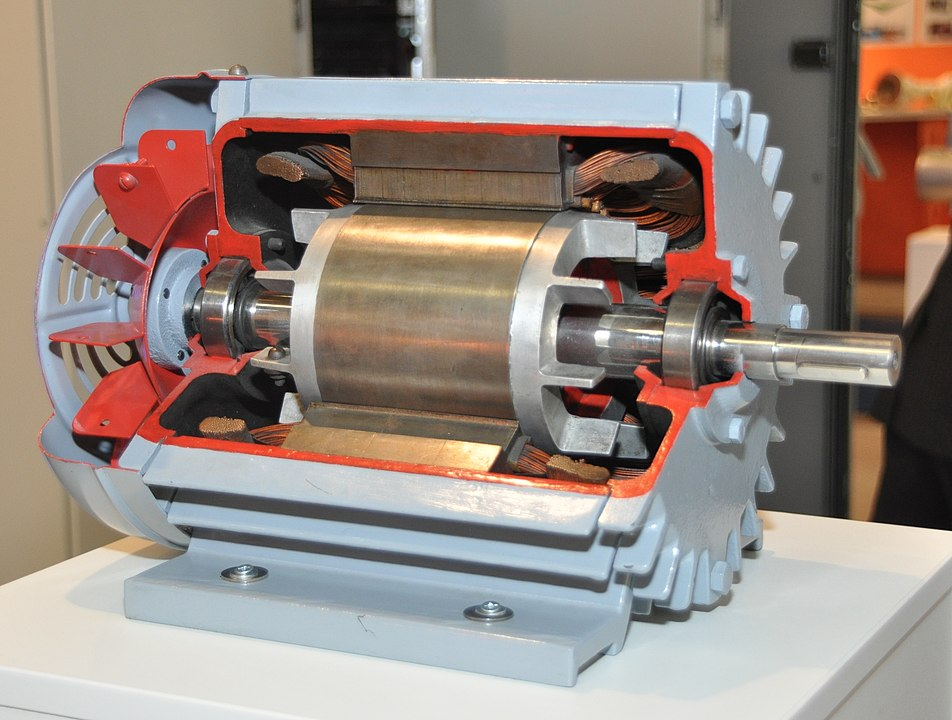
\includegraphics[width=6cm]{wikimedia-induction-motor.jpeg}\\
    {\footnotesize Source: S.J.~de~Ward, Wikimedia CC BY-SA 3.0}
  \end{center}

\end{frame}


\begin{frame}{The traveling flux wave of a four-pole motor}

  \begin{center}
    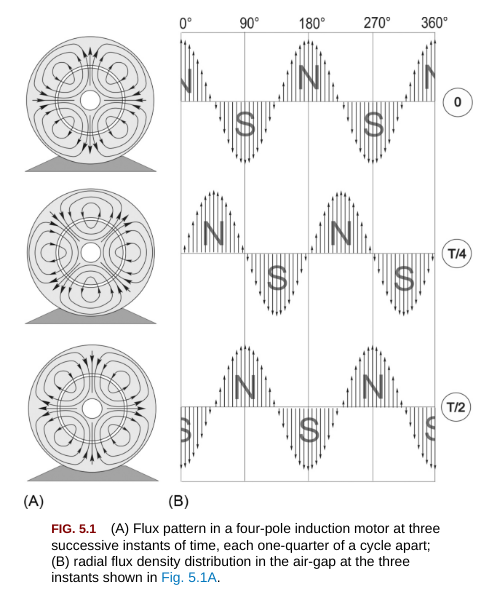
\includegraphics[width=6cm]{HD-fig5_1.png}\\
    {\footnotesize Source: Hughes and Drury}
  \end{center}

\end{frame}



% ---------------------------------------------------------
%
% Stator with slots, two slots per phase.
% Pulsating current. 
%
% ---------------------------------------------------------

\begin{frame}{Magnetic field generated by the stator winding currents}

  \begin{center}

    \begin{animateinline}[controls,autoplay,loop]{20}
      \multiframe{30}{n=1+12}{
        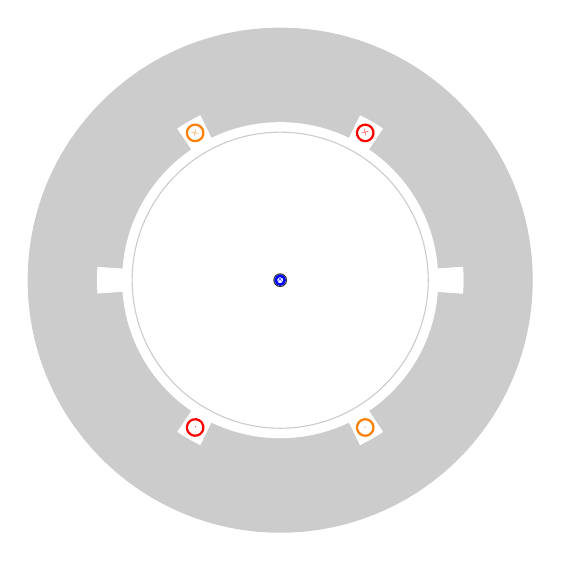
\begin{tikzpicture}[scale=0.4, transform shape]
          \pgfmathsetmacro{\slot}{8}
          \pgfmathsetmacro{\halfslot}{\slot/2}
          \pgfmathsetmacro{\outerrad}{50 + \slot}
          \draw[fill, black!20] (0, 0) circle[radius=80mm];
          \draw[fill, white] (0, 0) circle[radius=50mm];
          \foreach \rr in  {0,60,120,...,360} {
          \begin{scope}[rotate=\rr-\halfslot]
            \pgfmathsetmacro{\innerx}{50*cos(\slot)}
            \pgfmathsetmacro{\innery}{50*sin(\slot)}
            \draw[fill, white] (50 mm, 0) -- ++(\slot mm, 0) arc[start angle=0, end angle=\slot, radius=\outerrad mm] -- (\innerx mm, \innery mm) arc[start angle=\slot, end angle=0, radius=50mm];
          \end{scope}
          }
          \draw[black!20] (0, 0) circle[radius=47mm];
          \draw[black!80] (0, 0) circle[radius=2mm];
          \foreach \rr/\ph/\clr in {0/0/blue, 120/120/orange, -120/-120/red} {
            \pgfmathsetmacro{\current}{sin(\n + \ph)}
            \pgfmathsetmacro{\aa}{\halfslot*(1+abs(\current))}
            \pgfmathsetmacro{\cdir}{sign(\current)}
            \pgfmathsetmacro{\posx}{\cdir*(50 + \halfslot)}
            \pgfmathsetmacro{\negx}{-\posx}
            \begin{scope}[rotate=\rr]
              
              \draw[\clr,thick] (\posx mm, 0)  circle[radius=\aa pt];
              \node[] at (\posx mm, 0) {\textcolor{\clr}{$\times$}};
              \draw[\clr,thick] (\negx mm, 0)  circle[radius=\aa pt];
              \node[] at (\negx mm, 0) {\textcolor{\clr}{$\cdot$}};
              
            \end{scope}
          }
        \end{tikzpicture}    
      }
    \end{animateinline}
  \end{center}
\end{frame}

%---------------------------------------------------------
%
% Stator with slots, two slots per phase.
% Pulsating current. 
% Flux wave, one phase only
% ---------------------------------------------------------
\begin{frame}{Magnetic field generated by the stator winding currents}

  \begin{center}

    \begin{animateinline}[controls,autoplay,loop]{20}
      \multiframe{30}{n=1+12}{
        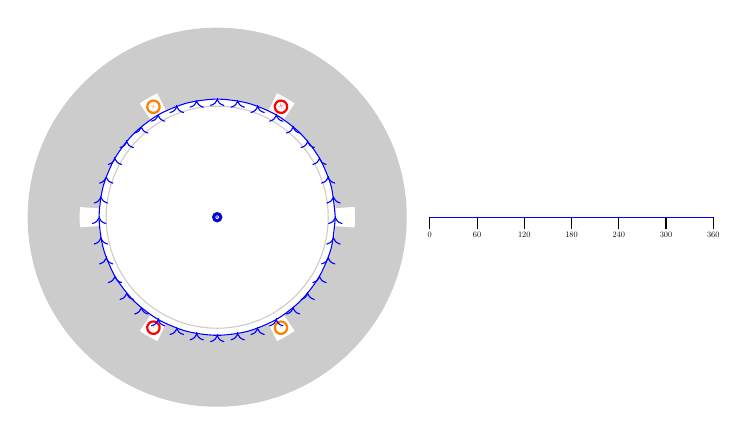
\begin{tikzpicture}[scale=0.3, transform shape]

          \begin{scope}[xshift = 8cm,]
            \pgfmathsetmacro{\axl}{12}
            \draw[] (0 cm, 0) -- (\axl cm, 0);
            \foreach \ax in {0, 60, 120, ..., 360} {
              \pgfmathsetmacro{\axx}{\ax*\axl/360.0)}
              \draw (\axx cm, 0) -- (\axx cm, -0.5) node[below] {\ax};
            }
            \foreach \rr/\ph/\clr in {0/0/blue} {
              \pgfmathsetmacro{\aa}{2*sin(\n + \ph)}
              \draw[\clr, domain=0:360, smooth, variable=\t]
              plot ( { \t*\axl/360.0 }, {\aa*cos(\t - 90 - \rr)} );
           }

          \end{scope}

          \begin{scope}[xshift=-1cm,]

            \pgfmathsetmacro{\slot}{8}
          \pgfmathsetmacro{\halfslot}{\slot/2}
          \pgfmathsetmacro{\outerrad}{50 + \slot}
          \draw[fill, black!20] (0, 0) circle[radius=80mm];
          \draw[fill, white] (0, 0) circle[radius=50mm];
          \foreach \rr in  {0,60,120,...,360} {
          \begin{scope}[rotate=\rr-\halfslot]
            \pgfmathsetmacro{\innerx}{50*cos(\slot)}
            \pgfmathsetmacro{\innery}{50*sin(\slot)}
            \draw[fill, white] (50 mm, 0) -- ++(\slot mm, 0) arc[start angle=0, end angle=\slot, radius=\outerrad mm] -- (\innerx mm, \innery mm) arc[start angle=\slot, end angle=0, radius=50mm];
          \end{scope}
          }
          \draw[black!20] (0, 0) circle[radius=47mm];
          \draw[black!80] (0, 0) circle[radius=2mm];

          \foreach \rr/\ph/\clr in {0/0/blue, 120/120/orange, -120/-120/red} {
            \pgfmathsetmacro{\current}{sin(\n + \ph)}
            \pgfmathsetmacro{\aa}{\halfslot*(1+abs(\current))}
            \pgfmathsetmacro{\cdir}{sign(\current)}
            \pgfmathsetmacro{\posx}{\cdir*(50 + \halfslot)}
            \pgfmathsetmacro{\negx}{-\posx}
            \begin{scope}[rotate=\rr]
              
              \draw[\clr,thick] (\posx mm, 0)  circle[radius=\aa pt];
              \node[] at (\posx mm, 0) {\textcolor{\clr}{$\times$}};
              \draw[\clr,thick] (\negx mm, 0)  circle[radius=\aa pt];
              \node[] at (\negx mm, 0) {\textcolor{\clr}{$\cdot$}};
              
            \end{scope}
          }
          \foreach \rr/\ph/\clr in {0/0/blue} {
            \begin{scope}[rotate=\rr, transform shape]

              \pgfmathsetmacro{\aa}{1*sin(\n + \ph)}
              \draw[\clr, domain=0:360, smooth, variable=\t]
               plot ( { (5+\aa*cos(\t-90))*cos(\t)}, {(5 + \aa*cos(\t - 90))*sin(\t)} );

               \foreach \aaa in {10,20,...,360} {
                 \pgfmathsetmacro{\vmag}{\aa*cos(\aaa-90)}
                 \pgfmathsetmacro{\xstart}{5*cos(\aaa)}
                 \pgfmathsetmacro{\ystart}{5*sin(\aaa)}
                 \pgfmathsetmacro{\xend}{(5+\vmag)*cos(\aaa)}
                 \pgfmathsetmacro{\yend}{(5+\vmag)*sin(\aaa)}

                 \draw[\clr, thin, ->] (\xstart, \ystart) to (\xend, \yend);
                 }
                 
             \end{scope}
          }
        \end{scope}

          
        \end{tikzpicture}    
      }
    \end{animateinline}
  \end{center}
\end{frame}

%\end{document}
% ---------------------------------------------------------
%
% Stator with slots, two slots per phase.
% Pulsating current. 
% Flux wave. Three phases
% ---------------------------------------------------------
\begin{frame}{Magnetic field generated by the stator winding currents}

  \begin{center}

    \begin{animateinline}[controls,autoplay,loop]{20}
      \multiframe{30}{n=1+12}{
        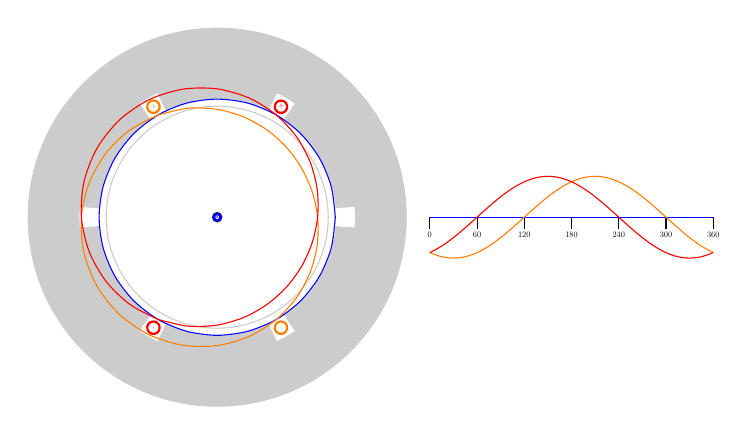
\begin{tikzpicture}[scale=0.3, transform shape]

          \begin{scope}[xshift = 8cm,]
            \pgfmathsetmacro{\axl}{12}
            \draw[] (0 cm, 0) -- (\axl cm, 0);
            \foreach \ax in {0, 60, 120, ..., 360} {
              \pgfmathsetmacro{\axx}{\ax*\axl/360.0)}
              \draw (\axx cm, 0) -- (\axx cm, -0.5) node[below] {\ax};
            }
            \foreach \rr/\ph/\clr in {0/0/blue, 120/120/orange, -120/-120/red} {
              \pgfmathsetmacro{\aa}{2*sin(\n + \ph)}
              \draw[\clr, domain=0:360, smooth, variable=\t]
              plot ( { \t*\axl/360.0 }, {\aa*cos(\t - 90 - \rr)} );
           }

          \end{scope}

          \begin{scope}[xshift=-1cm,]

            \pgfmathsetmacro{\slot}{8}
          \pgfmathsetmacro{\halfslot}{\slot/2}
          \pgfmathsetmacro{\outerrad}{50 + \slot}
          \draw[fill, black!20] (0, 0) circle[radius=80mm];
          \draw[fill, white] (0, 0) circle[radius=50mm];
          \foreach \rr in  {0,60,120,...,360} {
          \begin{scope}[rotate=\rr-\halfslot]
            \pgfmathsetmacro{\innerx}{50*cos(\slot)}
            \pgfmathsetmacro{\innery}{50*sin(\slot)}
            \draw[fill, white] (50 mm, 0) -- ++(\slot mm, 0) arc[start angle=0, end angle=\slot, radius=\outerrad mm] -- (\innerx mm, \innery mm) arc[start angle=\slot, end angle=0, radius=50mm];
          \end{scope}
          }
          \draw[black!20] (0, 0) circle[radius=47mm];
          \draw[black!80] (0, 0) circle[radius=2mm];

          \foreach \rr/\ph/\clr in {0/0/blue, 120/120/orange, -120/-120/red} {
            \pgfmathsetmacro{\current}{sin(\n + \ph)}
            \pgfmathsetmacro{\aa}{\halfslot*(1+abs(\current))}
            \pgfmathsetmacro{\cdir}{sign(\current)}
            \pgfmathsetmacro{\posx}{\cdir*(50 + \halfslot)}
            \pgfmathsetmacro{\negx}{-\posx}
            \begin{scope}[rotate=\rr]
              
              \draw[\clr,thick] (\posx mm, 0)  circle[radius=\aa pt];
              \node[] at (\posx mm, 0) {\textcolor{\clr}{$\times$}};
              \draw[\clr,thick] (\negx mm, 0)  circle[radius=\aa pt];
              \node[] at (\negx mm, 0) {\textcolor{\clr}{$\cdot$}};
              
            \end{scope}
          }
          \foreach \rr/\ph/\clr in {0/0/blue, 120/120/orange, -120/-120/red} {
            \begin{scope}[rotate=\rr, transform shape]

              \pgfmathsetmacro{\aa}{1*sin(\n + \ph)}
              \draw[\clr, domain=0:360, smooth, variable=\t]
               plot ( { (5+\aa*cos(\t-90))*cos(\t)}, {(5 + \aa*cos(\t - 90))*sin(\t)} );
            \end{scope}
          }
        \end{scope}

          
        \end{tikzpicture}    
      }
    \end{animateinline}
  \end{center}
\end{frame}

% ---------------------------------------------------------
%
% Stator with slots, two slots per phase.
% Pulsating current. 
% Flux wave. Three phases and resulting wave
% ---------------------------------------------------------
\begin{frame}{The air gap flux wave}

  The flux wave travels at the synchronous speed $N_s$ w.r.t.~the stator
  \[ N_s = \frac{120f}{p},\]
  where $f$ is the frequency of the AC power supply and $p$ is the pole number.
  
  \begin{center}

    \begin{animateinline}[controls,autoplay,loop]{20}
      \multiframe{30}{n=1+12}{
        \begin{tikzpicture}[scale=0.3, transform shape]

          \begin{scope}[xshift = 8cm,]
            \pgfmathsetmacro{\axl}{12}
            \draw[] (0 cm, 0) -- (\axl cm, 0);
            \foreach \ax in {0, 60, 120, ..., 360} {
              \pgfmathsetmacro{\axx}{\ax*\axl/360.0)}
              \draw (\axx cm, 0) -- (\axx cm, -0.5) node[below] {\ax};
            }
            \foreach \rr/\ph/\clr in {0/0/blue, 120/120/orange, -120/-120/red} {
              \pgfmathsetmacro{\aa}{2*sin(\n + \ph)}
              \draw[\clr!60, domain=0:360, smooth, variable=\t]
              plot ( { \t*\axl/360.0 }, {\aa*cos(\t - 90 - \rr)} );
            }
            
            \draw[black!80, domain=0:360, smooth, variable=\t]
            plot ( { \t*\axl/360.0 }, {2*(sin(\n)*cos(\t - 90 - 0) + sin(\n+120)*cos(\t - 90 - 120) + sin(\n-120)*cos(\t - 90 + 120)) } );

          \end{scope}

          \begin{scope}[xshift=-1cm,]

            \pgfmathsetmacro{\slot}{8}
          \pgfmathsetmacro{\halfslot}{\slot/2}
          \pgfmathsetmacro{\outerrad}{50 + \slot}
          \draw[fill, black!20] (0, 0) circle[radius=80mm];
          \draw[fill, white] (0, 0) circle[radius=50mm];
          \foreach \rr in  {0,60,120,...,360} {
          \begin{scope}[rotate=\rr-\halfslot]
            \pgfmathsetmacro{\innerx}{50*cos(\slot)}
            \pgfmathsetmacro{\innery}{50*sin(\slot)}
            \draw[fill, white] (50 mm, 0) -- ++(\slot mm, 0) arc[start angle=0, end angle=\slot, radius=\outerrad mm] -- (\innerx mm, \innery mm) arc[start angle=\slot, end angle=0, radius=50mm];
          \end{scope}
          }
          \draw[black!20] (0, 0) circle[radius=47mm];
          \draw[black!80] (0, 0) circle[radius=2mm];

          \foreach \rr/\ph/\clr in {0/0/blue, 120/120/orange, -120/-120/red} {
            \pgfmathsetmacro{\current}{sin(\n + \ph)}
            \pgfmathsetmacro{\aa}{\halfslot*(1+abs(\current))}
            \pgfmathsetmacro{\cdir}{sign(\current)}
            \pgfmathsetmacro{\posx}{\cdir*(50 + \halfslot)}
            \pgfmathsetmacro{\negx}{-\posx}
            \begin{scope}[rotate=\rr]
              
              \draw[\clr,thick] (\posx mm, 0)  circle[radius=\aa pt];
              \node[] at (\posx mm, 0) {\textcolor{\clr}{$\times$}};
              \draw[\clr,thick] (\negx mm, 0)  circle[radius=\aa pt];
              \node[] at (\negx mm, 0) {\textcolor{\clr}{$\cdot$}};
              
            \end{scope}
          }
          \foreach \rr/\ph/\clr in {0/0/blue, 120/120/orange, -120/-120/red} {
            \begin{scope}[rotate=\rr, transform shape]
              \pgfmathsetmacro{\aa}{1*sin(\n + \ph)}

              \draw[\clr!60, domain=0:360, smooth, variable=\t]
               plot ( { (5+\aa*cos(\t-90))*cos(\t)}, {(5 + \aa*cos(\t - 90))*sin(\t)} );
            \end{scope}
          }
          \draw[black!80, domain=0:360, smooth, variable=\t]
            plot ( { (5 + ( sin(\n)*cos(\t - 90 - 0) + sin(\n+120)*cos(\t - 90 - 120) + sin(\n-120)*cos(\t - 90 + 120)))*cos(\t)}, {(5 + (sin(\n)*cos(\t - 90 - 0) + sin(\n+120)*cos(\t - 90 - 120) + sin(\n-120)*cos(\t - 90 + 120)))*sin(\t) });

        \end{scope}

          
        \end{tikzpicture}    
      }
    \end{animateinline}
  \end{center}
\end{frame}

% ---------------------------------------------------------
%
% Stator with slots, two slots per phase.
% Pulsating current. 
% Flux wave. Three phases and resulting wave
% ---------------------------------------------------------
\begin{frame}{The air gap flux wave}

  \begin{center}

    \begin{animateinline}[controls,autoplay,loop]{20}
      \multiframe{30}{n=1+12}{
        \begin{tikzpicture}[scale=0.3, transform shape]

          \begin{scope}[xshift = 8cm,]
            \pgfmathsetmacro{\axl}{12}
            \draw[] (0 cm, 0) -- (\axl cm, 0);
            \foreach \ax in {0, 60, 120, ..., 360} {
              \pgfmathsetmacro{\axx}{\ax*\axl/360.0)}
              \draw (\axx cm, 0) -- (\axx cm, -0.5) node[below] {\ax};
            }
            \foreach \rr/\ph/\clr in {0/0/blue, 120/120/orange, -120/-120/red} {
              \pgfmathsetmacro{\aa}{2*sin(\n + \ph)}
              \draw[\clr!40, domain=0:360, smooth, variable=\t]
              plot ( { \t*\axl/360.0 }, {\aa*cos(\t - 90 - \rr)} );
            }
            
            \draw[black!80, domain=0:360, smooth, variable=\t]
            plot ( { \t*\axl/360.0 }, {2*(sin(\n)*cos(\t - 90 - 0) + sin(\n+120)*cos(\t - 90 - 120) + sin(\n-120)*cos(\t - 90 + 120)) } );

          \end{scope}

          \begin{scope}[xshift=-1cm,]

            \pgfmathsetmacro{\slot}{8}
          \pgfmathsetmacro{\halfslot}{\slot/2}
          \pgfmathsetmacro{\outerrad}{50 + \slot}
          \draw[fill, black!20] (0, 0) circle[radius=80mm];
          \draw[fill, white] (0, 0) circle[radius=50mm];
          \foreach \rr in  {0,60,120,...,360} {
          \begin{scope}[rotate=\rr-\halfslot]
            \pgfmathsetmacro{\innerx}{50*cos(\slot)}
            \pgfmathsetmacro{\innery}{50*sin(\slot)}
            \draw[fill, white] (50 mm, 0) -- ++(\slot mm, 0) arc[start angle=0, end angle=\slot, radius=\outerrad mm] -- (\innerx mm, \innery mm) arc[start angle=\slot, end angle=0, radius=50mm];
          \end{scope}
          }
          \draw[black!20] (0, 0) circle[radius=47mm];
          \draw[black!80] (0, 0) circle[radius=2mm];

          \foreach \rr/\ph/\clr in {0/0/blue, 120/120/orange, -120/-120/red} {
            \pgfmathsetmacro{\current}{sin(\n + \ph)}
            \pgfmathsetmacro{\aa}{\halfslot*(1+abs(\current))}
            \pgfmathsetmacro{\cdir}{sign(\current)}
            \pgfmathsetmacro{\posx}{\cdir*(50 + \halfslot)}
            \pgfmathsetmacro{\negx}{-\posx}
            \begin{scope}[rotate=\rr]
              
              \draw[\clr,thick] (\posx mm, 0)  circle[radius=\aa pt];
              \node[] at (\posx mm, 0) {\textcolor{\clr}{$\times$}};
              \draw[\clr,thick] (\negx mm, 0)  circle[radius=\aa pt];
              \node[] at (\negx mm, 0) {\textcolor{\clr}{$\cdot$}};
              
            \end{scope}
          }
          \draw[black!80, domain=0:360, smooth, variable=\t]
            plot ( { (5 + ( sin(\n)*cos(\t - 90 - 0) + sin(\n+120)*cos(\t - 90 - 120) + sin(\n-120)*cos(\t - 90 + 120)))*cos(\t)}, {(5 + (sin(\n)*cos(\t - 90 - 0) + sin(\n+120)*cos(\t - 90 - 120) + sin(\n-120)*cos(\t - 90 + 120)))*sin(\t) });

        \end{scope}

          
        \end{tikzpicture}    
      }
    \end{animateinline}
  \end{center}
\end{frame}

% ---------------------------------------------------------
%
% 4-pole Stator with slots, two slots per phase.
% Pulsating current. 
% Flux wave. Three phases and resulting wave
% ---------------------------------------------------------
\begin{frame}{The air gap flux wave for a 4-pole motor}

  \begin{center}

    \begin{animateinline}[controls,autoplay,loop]{20}
      \multiframe{30}{n=1+12}{
        \begin{tikzpicture}[scale=0.3, transform shape]

          \begin{scope}[xshift = 8cm,]
            \pgfmathsetmacro{\axl}{12}
            \draw[] (0 cm, 0) -- (\axl cm, 0);
            \foreach \ax in {0, 60, 120, ..., 360} {
              \pgfmathsetmacro{\axx}{\ax*\axl/360.0)}
              \draw (\axx cm, 0) -- (\axx cm, -0.5) node[below] {\ax};
            }
            \foreach \rr/\ph/\clr in {0/0/blue, 120/120/orange, -120/-120/red} {
              \pgfmathsetmacro{\aa}{2*sin(\n + \ph)}
              \draw[\clr!40, domain=0:720, smooth, variable=\t]
              plot ( { \t*\axl/360.0/2 }, {\aa*cos(\t - 90 - \rr)} );
            }
            
            \draw[black!80, domain=0:720, smooth, variable=\t]
            plot ( { \t*\axl/360.0/2 }, {2*(sin(\n)*cos(\t - 90 - 0) + sin(\n+120)*cos(\t - 90 - 120) + sin(\n-120)*cos(\t - 90 + 120)) } );

          \end{scope}

          \begin{scope}[xshift=-1cm,]

            \pgfmathsetmacro{\slot}{8}
          \pgfmathsetmacro{\halfslot}{\slot/2}
          \pgfmathsetmacro{\outerrad}{50 + \slot}
          \draw[fill, black!20] (0, 0) circle[radius=80mm];
          \draw[fill, white] (0, 0) circle[radius=50mm];
          \foreach \rr in  {30,60,90,...,360} {
          \begin{scope}[rotate=\rr-\halfslot]
            \pgfmathsetmacro{\innerx}{50*cos(\slot)}
            \pgfmathsetmacro{\innery}{50*sin(\slot)}
            \draw[fill, white] (50 mm, 0) -- ++(\slot mm, 0) arc[start angle=0, end angle=\slot, radius=\outerrad mm] -- (\innerx mm, \innery mm) arc[start angle=\slot, end angle=0, radius=50mm];
          \end{scope}
          }
          \draw[black!20] (0, 0) circle[radius=47mm];
          \draw[black!80] (0, 0) circle[radius=2mm];

          \foreach \rr/\ph/\clr in {0/0/blue, 120/120/orange, -120/-120/red} {
            \pgfmathsetmacro{\current}{sin(\n + \ph)}
            \pgfmathtruncatemacro{\trunccurrent}{100*\current}
            \pgfmathsetmacro{\aa}{\halfslot*(1+abs(\current))}
            \pgfmathsetmacro{\cdir}{sign(\current)}
            \pgfmathsetmacro{\condmid}{(50 + \halfslot)}
            \begin{scope}[rotate=\rr]
              
              \draw[\clr,thick] (\condmid mm, 0)  circle[radius=\aa pt];
              \draw[\clr,thick] (-\condmid mm, 0)  circle[radius=\aa pt];
              \draw[\clr,thick] (0, \condmid mm)  circle[radius=\aa pt];
              \draw[\clr,thick] (0, -\condmid mm)  circle[radius=\aa pt];

              %\ifthenelse{ \trunccurrent > 0}
              %{%
              %  \draw[fill, \clr] (\condmid mm, 0) circle[radius = 2pt];
              %  \draw[fill, \clr] (-\condmid mm, 0) circle[radius = 2pt];
              %  \draw[\clr] (0, \condmid mm, 0) ++ (-4pt, -4pt) -- ++(8pt, 8pt) ++ (-8pt, 0pt) -- ++(8pt, -8pt);
              %  \draw[\clr] (0, -\condmid mm) ++ (-4pt, -4pt) -- ++(8pt, 8pt) ++ (-8pt, 0pt) -- ++(8pt, -8pt);}
              %{%
              %  \draw[fill, \clr] (0, \condmid mm, 0) circle[radius = 2pt];
              %  \draw[fill, \clr] (0, -\condmid mm) circle[radius = 2pt];
              %  \draw[\clr] (\condmid mm, 0) ++ (-4pt, -4pt) -- ++(8pt, 8pt) ++ (-8pt, 0pt) -- ++(8pt, -8pt);
              %  \draw[\clr] (-\condmid mm, 0) ++ (-4pt, -4pt) -- ++(8pt, 8pt) ++ (-8pt, 0pt) -- ++(8pt, -8pt);}

            \end{scope}
          }
          \draw[black!80, domain=0:720, smooth, variable=\t]
            plot ( { (5 + ( sin(\n)*cos(\t - 90 - 0) + sin(\n+120)*cos(\t - 90 - 120) + sin(\n-120)*cos(\t - 90 + 120)))*cos(\t/2)}, {(5 + (sin(\n)*cos(\t - 90 - 0) + sin(\n+120)*cos(\t - 90 - 120) + sin(\n-120)*cos(\t - 90 + 120)))*sin(\t/2) });

        \end{scope}

          
        \end{tikzpicture}    
      }
    \end{animateinline}
  \end{center}
\end{frame}


\begin{frame}{E.m.f.~generated by a moving magnetic field}
\begin{center}
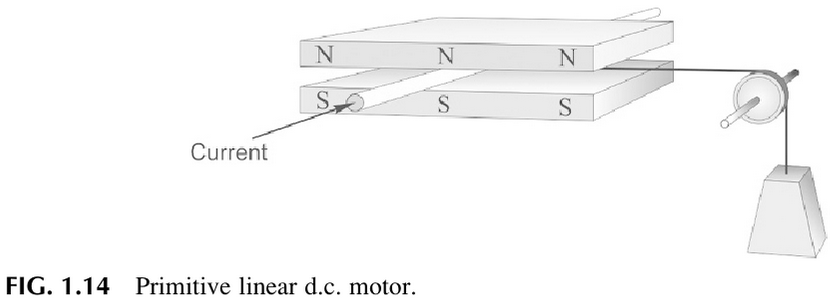
\includegraphics[width=5cm]{HD-fig1_14.png}
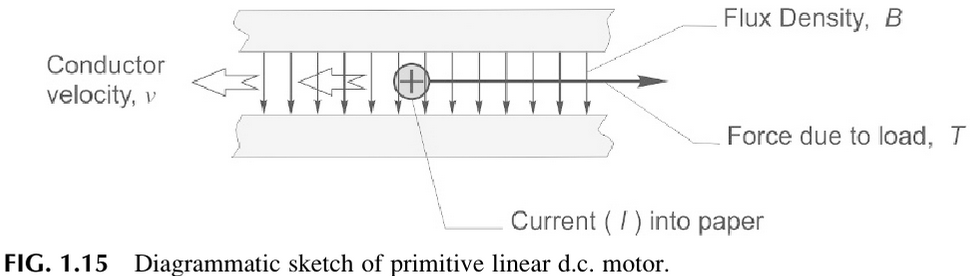
\includegraphics[width=5cm]{HD-fig1_15.png}\\
{\footnotesize Source: Hughes and Drury}
\end{center}

In the primitive linear motor with conductor moving at velocity $v$ w.r.t~ the magnetic field, the (back) e.m.f.~is proportional to the velocity $v$ and the flux density $B$.

\end{frame}


% ---------------------------------------------------------
%
% Stator without slots, Rotor with cage.
% Traveling flux wave.
%---------------------------------------------------------
\begin{frame}{The effect of the air gap flux wave on the rotor}

  The rotor rotates at speed $N =(1-s)N_s< N_s$, where the slip is defined as $s=\frac{N_s-N}{N_s}$. The reference frame is fixed in the rotor. The flux wave travels at the slip speed $sN_s$ w.r.t~the rotor.
  
  \begin{center}

    \begin{animateinline}[controls,autoplay,loop]{10}
      \multiframe{30}{n=1+12}{
        \begin{tikzpicture}[scale=0.3, transform shape]

          \begin{scope}[xshift = 8cm,]
            \pgfmathsetmacro{\axl}{12}
            \draw[] (0 cm, 0) -- (\axl cm, 0);
            \foreach \ax in {0, 60, 120, ..., 360} {
              \pgfmathsetmacro{\axx}{\ax*\axl/360.0)}
              \draw (\axx cm, 0) -- (\axx cm, -0.5) node[below] {\ax};
            }
            \draw[black!80, domain=0:720, smooth, variable=\t]
            plot ( { \t*\axl/360.0/2 }, {2*(sin(\n)*cos(\t - 90 - 0) + sin(\n+120)*cos(\t - 90 - 120) + sin(\n-120)*cos(\t - 90 + 120)) } );

          \end{scope}

          \begin{scope}[xshift=-1cm,]

            \pgfmathsetmacro{\rodradius}{3}
            \pgfmathsetmacro{\cageradius}{47-\rodradius}
          \draw[fill, black!20] (0, 0) circle[radius=80mm];
          \draw[fill, white] (0, 0) circle[radius=50mm];
          \draw[fill, black!10] (0, 0) circle[radius=47mm];
          \foreach \rr in  {15,30,45,...,360} {
          \begin{scope}[rotate=\rr]
            \draw[fill, black!60] (\cageradius mm, 0) circle[radius=\rodradius mm];
          \end{scope}
          }
          \draw[black!80] (0, 0) circle[radius=2mm];

          \draw[black!80, domain=0:720, smooth, variable=\t]
            plot ( { (5 + ( sin(\n)*cos(\t - 90 - 0) + sin(\n+120)*cos(\t - 90 - 120) + sin(\n-120)*cos(\t - 90 + 120)))*cos(\t/2)}, {(5 + (sin(\n)*cos(\t - 90 - 0) + sin(\n+120)*cos(\t - 90 - 120) + sin(\n-120)*cos(\t - 90 + 120)))*sin(\t/2) });

        \end{scope}

          
        \end{tikzpicture}    
      }
    \end{animateinline}
  \end{center}
\end{frame}

%\end{document}

% ---------------------------------------------------------
%
% Stator without slots, Rotor with cage.
% Traveling flux wave.
% Induced current
% ---------------------------------------------------------
\begin{frame}{Induced currents in the rotor, small slip}

  Flux wave shown in black, induced e.m.f shown in green and induced rotor current shown in magenta.
  \begin{center}

    \begin{animateinline}[controls,autoplay,loop]{10}
      \multiframe{30}{n=1+12}{
        \begin{tikzpicture}[scale=0.3, transform shape]

          \pgfmathsetmacro{\clag}{10}
          \begin{scope}[xshift = 8cm,]
            \pgfmathsetmacro{\axl}{12}
            \draw[] (0 cm, 0) -- (\axl cm, 0);
            \foreach \ax in {0, 60, 120, ..., 360} {
              \pgfmathsetmacro{\axx}{\ax*\axl/360.0)}
              \draw (\axx cm, 0) -- (\axx cm, -0.5) node[below] {\ax};
            }
            \draw[black!80, domain=0:720, smooth, variable=\t]
            plot ( { \t*\axl/360.0/2 }, {2*(sin(\n)*cos(\t - 90 - 0) + sin(\n+120)*cos(\t - 90 - 120) + sin(\n-120)*cos(\t - 90 + 120)) } );

            \draw[green!70!black, domain=0:720, smooth, variable=\t]
            plot ( { \t*\axl/360.0/2 }, {1.7*(sin(\n)*cos(\t - 90 - 0) + sin(\n+120)*cos(\t - 90 - 120) + sin(\n-120)*cos(\t - 90 + 120)) } );

            \draw[magenta, domain=0:720, smooth, variable=\t]
            plot ( { \t*\axl/360.0/2 }, {1.2*(sin(\n)*cos(\t -\clag - 90 - 0) + sin(\n+120)*cos(\t -\clag - 90 - 120) + sin(\n-120)*cos(\t -\clag - 90 + 120)) } );

          \end{scope}

          \begin{scope}[xshift=-1cm,]

            \pgfmathsetmacro{\rodradius}{3}
            \pgfmathsetmacro{\cageradius}{47-\rodradius}
          \draw[fill, black!20] (0, 0) circle[radius=80mm];
          \draw[fill, white] (0, 0) circle[radius=50mm];
          \draw[fill, black!10] (0, 0) circle[radius=47mm];

          \foreach \rr in  {15,30,45,...,360} {
          \begin{scope}[rotate=\rr]
            \pgfmathsetmacro{\current}{sin(\n)*cos(2*\rr -\clag - 90 - 0) + sin(\n+120)*cos(2*\rr -\clag - 90 - 120) + sin(\n-120)*cos(2*\rr -\clag - 90 + 120)}
            \pgfmathtruncatemacro{\trunccurrent}{100*\current}
            \pgfmathsetmacro{\inducedcurrent}{3*abs(\current)}
            \draw[fill, magenta] (\cageradius mm, 0) circle[radius=\inducedcurrent mm];
            \ifthenelse{\trunccurrent > 0}{%
              \draw[fill, black] (\cageradius mm, 0) circle[radius = 1pt];}{%
              \draw[black] (\cageradius mm, 0) ++ (-4pt, -4pt) -- ++(8pt, 8pt) ++ (-8pt, 0pt) -- ++(8pt, -8pt);}
          \end{scope}
          }
          \draw[black!80] (0, 0) circle[radius=2mm];

          \draw[black!80, domain=0:720, smooth, variable=\t]
            plot ( { (5 + ( sin(\n)*cos(\t - 90 - 0) + sin(\n+120)*cos(\t - 90 - 120) + sin(\n-120)*cos(\t - 90 + 120)))*cos(\t/2)}, {(5 + (sin(\n)*cos(\t - 90 - 0) + sin(\n+120)*cos(\t - 90 - 120) + sin(\n-120)*cos(\t - 90 + 120)))*sin(\t/2) });

            \foreach \aaa in {10,20,...,360} {
              \pgfmathsetmacro{\vmag}{( sin(\n)*cos(2*\aaa - 90 - 0) + sin(\n+120)*cos(2*\aaa - 90 - 120) + sin(\n-120)*cos(2*\aaa - 90 + 120))}
              \pgfmathsetmacro{\xstart}{5*cos(\aaa)}
              \pgfmathsetmacro{\ystart}{5*sin(\aaa)}
              \pgfmathsetmacro{\xend}{(5+\vmag)*cos(\aaa)}
              \pgfmathsetmacro{\yend}{(5+\vmag)*sin(\aaa)}
              
              \draw[black, thin, ->] (\xstart, \ystart) to (\xend, \yend);
            }
            
        \end{scope}

          
        \end{tikzpicture}    
      }
    \end{animateinline}
  \end{center}
\end{frame}

\end{document}

----------------------------------------------
% Vectors
% ----------------------------------------------

\begin{frame}{Magnetic field generated by the stator winding currents}

  \begin{center}

    \begin{animateinline}[controls,autoplay,loop]{20}
      \multiframe{30}{n=1+12}{
        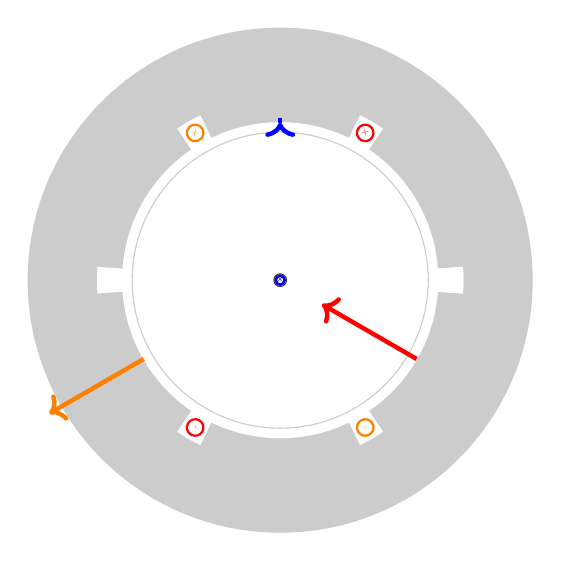
\begin{tikzpicture}[scale=0.4, transform shape]
          \pgfmathsetmacro{\slot}{8}
          \pgfmathsetmacro{\halfslot}{\slot/2}
          \pgfmathsetmacro{\outerrad}{50 + \slot}
          \draw[fill, black!20] (0, 0) circle[radius=80mm];
          \draw[fill, white] (0, 0) circle[radius=50mm];
          \foreach \rr in  {0,60,120,...,360} {
          \begin{scope}[rotate=\rr-\halfslot]
            \pgfmathsetmacro{\innerx}{50*cos(\slot)}
            \pgfmathsetmacro{\innery}{50*sin(\slot)}
            \draw[fill, white] (50 mm, 0) -- ++(\slot mm, 0) arc[start angle=0, end angle=\slot, radius=\outerrad mm] -- (\innerx mm, \innery mm) arc[start angle=\slot, end angle=0, radius=50mm];
          \end{scope}
          }
          \draw[black!20] (0, 0) circle[radius=47mm];
          \draw[black!80] (0, 0) circle[radius=2mm];
          \foreach \rr/\ph/\clr in {0/0/blue, 120/120/orange, -120/-120/red} {
            \pgfmathsetmacro{\current}{sin(\n + \ph)}
            \pgfmathsetmacro{\aa}{\halfslot*(1+abs(\current))}
            \pgfmathsetmacro{\cdir}{sign(\current)}
            \pgfmathsetmacro{\posx}{\cdir*(50 + \halfslot)}
            \pgfmathsetmacro{\negx}{-\posx}
            \begin{scope}[rotate=\rr]
              
              \draw[\clr,thick] (\posx mm, 0)  circle[radius=\aa pt];
              \node[] at (\posx mm, 0) {\textcolor{\clr}{$\times$}};
              \draw[\clr,thick] (\negx mm, 0)  circle[radius=\aa pt];
              \node[] at (\negx mm, 0) {\textcolor{\clr}{$\cdot$}};
              
            \end{scope}
          }
          \foreach \rr/\ph/\clr in {0/0/blue, 120/120/orange, -120/-120/red} {
            \begin{scope}[rotate=\rr, transform shape]
              \pgfmathsetmacro{\aa}{4*sin(\n + \ph)}
              \draw[\clr, ->, ultra thick] (0,5) -- ++ (0,\aa);
            \end{scope}
          }
          
        \end{tikzpicture}    
      }
    \end{animateinline}
  \end{center}
\end{frame}

\end{document}

\begin{frame}{Rotating magnetic field}

  \begin{center}

    \begin{animateinline}[controls,autoplay,loop]{20}
\multiframe{30}{n=0+12}{
  \begin{tikzpicture}[scale=0.4, transform shape]
    \draw[black!20] (0, 0) circle[radius=47mm];
    \draw[black!80] (0, 0) circle[radius=2mm];
    \foreach \rr/\ph/\clr in {0/0/blue, 120/120/white, -120/-120/white} {
      \begin{scope}[rotate=\rr, transform shape]
        \pgfmathsetmacro{\aa}{4*sin(\n + \ph)}
        \draw (-1.5, 10) to[current source] (-1.5, 13) to[short] (0,13) to[L] (0, 10) to[short] (-1.5,10);
        \draw[\clr, ->, ultra thick] (0,5) -- ++ (0,\aa);
    \end{scope}
  }
  \end{tikzpicture}    
}
\end{animateinline}
\end{center}
\end{frame}

\begin{frame}{Rotating magnetic field}

  \begin{center}

    \begin{animateinline}[controls,autoplay,loop]{20}
\multiframe{30}{n=0+12}{
  \begin{tikzpicture}[scale=0.4, transform shape]
    \draw[black!20] (0, 0) circle[radius=47mm];
    \draw[black!80] (0, 0) circle[radius=2mm];
    \foreach \rr/\ph/\clr in {0/0/blue, 120/120/orange, -120/-120/red} {
      \begin{scope}[rotate=\rr, transform shape]
        \pgfmathsetmacro{\aa}{4*sin(\n + \ph)}
        \draw (-1.5, 10) to[current source] (-1.5, 13) to[short] (0,13) to[L] (0, 10) to[short] (-1.5,10);
        \draw[\clr, ->, ultra thick] (0,5) -- ++ (0,\aa);
    \end{scope}
  }
  \end{tikzpicture}    
}
\end{animateinline}
\end{center}
\end{frame}

\begin{frame}{Rotating magnetic field}

  \begin{center}

    \begin{animateinline}[controls,autoplay,loop]{10}
\multiframe{60}{n=0+6}{
  \begin{tikzpicture}[scale=0.4, transform shape]
    \draw[black!20] (0, 0) circle[radius=47mm];
    \draw[black!80] (0, 0) circle[radius=2mm];
    \foreach \rr in {0, 120, -120} {
      \begin{scope}[rotate=\rr, ]
        \draw (-1.5, 10) to[current source] (-1.5, 13) to[short] (0,13) to[L] (0, 10) to[short] (-1.5,10);
    \end{scope}
  }
    \pgfmathsetmacro{\aU}{4*sin(\n + 0)}
    \pgfmathsetmacro{\aV}{4*sin(\n + 120)}
    \pgfmathsetmacro{\aW}{4*sin(\n - 120)}
    \pgfmathsetmacro{\Ux}{0}
    \pgfmathsetmacro{\Uy}{\aU*cos(0)}
    \pgfmathsetmacro{\Vx}{\aV*sin(120)}
    \pgfmathsetmacro{\Vy}{\aV*cos(120)}
    \pgfmathsetmacro{\Wx}{\aW*sin(-120)}
    \pgfmathsetmacro{\Wy}{\aW*cos(-120)}
    \draw[blue, ->,  thick] (0,0) -- ++ (\Ux, \Uy);
    \draw[orange, ->,  thick] (0,0) ++ (\Ux, \Uy) -- ++ (\Vx, \Vy);
    \draw[red, ->,  thick] (0,0) ++ (\Ux, \Uy)  ++ (\Vx, \Vy) -- ++(\Wx, \Wy);
    \draw[black!80, <-,  thick] (0,0) ++ (\Ux, \Uy)  ++ (\Vx, \Vy) ++(\Wx, \Wy) -- (0,0);

  \end{tikzpicture}    
}
\end{animateinline}
\end{center}
\end{frame}

\end{document}